\documentclass[11pt,a4paper]{article}
\usepackage[utf8]{inputenc}
\usepackage[margin=1in]{geometry}
\usepackage{hyperref}
\usepackage{graphicx}
\usepackage{enumitem}
\usepackage{xcolor}
\usepackage{tcolorbox}
\usepackage{listings}
\usepackage{fancyhdr}
\usepackage{titlesec}
\usepackage{amssymb}
\usepackage{booktabs} % For better tables
\usepackage{float}    % For [H] positioning
\usepackage{CJKutf8}  % For Chinese characters support
\usepackage{fontawesome5} % For icons

% Configure listings for code syntax highlighting
\lstdefinestyle{pythonstyle}{
    language=Python,
    basicstyle=\ttfamily\small,
    keywordstyle=\color{blue}\bfseries,
    stringstyle=\color{red},
    commentstyle=\color{green!50!black}\itshape,
    backgroundcolor=\color{gray!5},
    frame=single,
    rulecolor=\color{gray!30},
    numbers=left,
    numberstyle=\tiny\color{gray},
    numbersep=5pt,
    breaklines=true,
    showstringspaces=false,
    tabsize=4,
    captionpos=b
}

\lstdefinestyle{bashstyle}{
    language=bash,
    basicstyle=\ttfamily\small\color{black},
    keywordstyle=\color{purple}\bfseries,
    commentstyle=\color{gray}\itshape,
    backgroundcolor=\color{blue!5},
    frame=leftline,
    framerule=3pt,
    rulecolor=\color{blue!50},
    numbers=none,
    breaklines=true,
    showstringspaces=false,
    tabsize=2
}

\lstset{
    basicstyle=\ttfamily\small,
    columns=flexible,
    breaklines=true
}

% Define custom itemize bullet commands
\newcommand{\gooditem}{\item[\color{green!70!black}\faCheck]}
\newcommand{\baditem}{\item[\color{red!70!black}\faTimes]}
\newcommand{\toolitem}{\item[\color{blue!70!black}\faCog]}
\newcommand{\ideaitem}{\item[\color{yellow!80!black}\faLightbulb]}
\newcommand{\warningitem}{\item[\color{orange}\faExclamationTriangle]}
\newcommand{\staritem}{\item[\color{goldenyellow}\faStar]}
\newcommand{\arrowitem}{\item[\color{darkblue}\faArrowRight]}

% Define colors
\definecolor{darkblue}{RGB}{0,0,139}
\definecolor{lightgray}{RGB}{240,240,240}
\definecolor{harvardcrimson}{RGB}{165,28,48}
\definecolor{emeraldgreen}{RGB}{0,155,119}
\definecolor{royalpurple}{RGB}{102,51,153}
\definecolor{goldenyellow}{RGB}{255,193,37}

% Header and footer
\pagestyle{fancy}
\setlength{\headheight}{14.5pt}
\fancyhf{}
\rhead{Student Research Excellence Guide}
\lhead{Research Handbook}
\rfoot{Page \thepage}

% Title formatting
\titleformat{\section}{\Large\bfseries\color{darkblue}}{\thesection}{1em}{}
\titleformat{\subsection}{\large\bfseries}{\thesubsection}{1em}{}

% Hyperlink setup
\hypersetup{
    colorlinks=true,
    linkcolor=darkblue,
    urlcolor=blue,
    citecolor=darkblue
}

\title{\textbf{New Researcher Handbook}\\
\large A Practical Guide for Early-Career PhD Students and Researchers}
\author{\href{https://aaronluo00.github.io/Aaron_Homepage/}{Xiaolong Luo}\\
Harvard University\\
School of Engineering and Applied Sciences\\
\vspace{0.5cm}
\small\textit{Also available on: \href{http://xhslink.com/m/5E5I3850qZP}{Xiaohongshu \begin{CJK}{UTF8}{gbsn}(小红书)\end{CJK}}}}
\date{\today}

\begin{document}

\maketitle

\tableofcontents
\newpage

\section{\faBook~Introduction}

\subsection{Why This Manual Matters}

Dear students,

\textbf{I wish I had seen this manual when I was an undergraduate student, or when I just started my PhD journey.} It would have saved me from countless detours, mistakes, and unnecessary struggles. This guide contains the lessons I learned the hard way—through trial and error, late-night debugging sessions, rejected papers, and awkward presentations.

Looking back, I realize how much time and energy I could have saved if someone had told me:
\begin{itemize}
    \ideaitem The importance of version control (I lost weeks of work because I didn't use Git properly)
    \ideaitem How to structure presentations (my first conference talk was a disaster—no clear message, too much detail)
    \ideaitem The value of documentation (I couldn't understand my own code from 6 months earlier)
    \ideaitem How to ask good questions in meetings (I stayed silent for months, missing valuable learning opportunities)
\end{itemize}

\textbf{These aren't just rules—they're shortcuts to success that I discovered too late:}
\begin{itemize}
    \gooditem Clear communication skills will help you share your ideas effectively
    \gooditem Rigorous research habits will make you a trusted and reliable researcher
    \gooditem Professional presentation skills will open doors to opportunities
    \gooditem Good documentation practices will save you countless hours in the future
    \gooditem Collaborative skills will make you a valued team member anywhere you go
\end{itemize}

As a PhD candidate in my fourth year, I'm still learning these lessons myself. Every guideline in this manual comes from mistakes I've made or witnessed firsthand. When I emphasize the importance of presentation skills, it's because I've missed many opportunities and left poor impressions due to bad presentations. When I emphasize documentation, it's because I've personally struggled to recreate my own experiments from months earlier.

The habits we develop now will serve us when we're:
\begin{itemize}
    \staritem Presenting at international conferences (where we have one shot to impress)
    \staritem Defending our theses (where clarity can make or break the defense)
    \staritem Interviewing for our dream jobs (where these skills set us apart)
    \staritem Eventually leading our own research teams (where we'll pass on these lessons)
    \staritem Pitching ideas to investors or stakeholders (where professionalism matters most)
\end{itemize}

\textbf{My intention is simple:} By sharing what I've learned so far in my PhD journey, I hope we can learn from each other's experiences. This manual isn't written from a position of mastery—it's a collection of lessons I'm still learning, mistakes I'm still making, and habits I'm still building. Let's navigate this journey together and help each other become the researchers we aspire to be.

\subsection{How We Build Research Excellence}

Beyond the technical skills, remember that excellence in research comes from:
\begin{itemize}
    \item \textbf{Frequent feedback from each other}: Don't work in isolation—share your work early and often
    \item \textbf{Reflecting on our personal and research practices}: Take time to think about what's working and what isn't
    \item \colorbox{yellow!30}{\textbf{Getting enough sleep so we can bring our best selves to our work}:} \newline \colorbox{yellow!30}{Exhausted researchers make poor decisions and write buggy code}
\end{itemize}

These principles might sound simple, but I've seen too many brilliant students burn out because they ignored them. Your best work comes when you're well-rested, connected with your community, and continuously learning from both successes and failures.

\section{\faGem~Core Principles}

\subsection{Clarity Above All}
Every presentation should prioritize clarity. Your audience should understand:
\begin{itemize}
    \item The problem you're solving
    \item Your approach
    \item Your results and their implications
\end{itemize}

\subsection{Consistency Matters}
Use consistent formatting, terminology, and structure throughout your presentations and reports.

\subsection{Respect Your Audience}
Remember that your audience's time is valuable. Be prepared, be concise, and be engaging.

\section{\faChalkboardTeacher~Presentation Standards}

\subsection{Structure}
Every presentation should follow this structure:
\begin{enumerate}
    \item \textbf{Title Slide}: Include title, your name, date, and affiliation
    \item \textbf{Outline}: Brief overview of what you'll cover
    \item \textbf{Background/Motivation}: Why this work matters
    \item \textbf{Problem Statement}: Clear definition of what you're solving
    \item \textbf{Methodology}: Your approach
    \item \textbf{Results}: What you found
    \item \textbf{Discussion}: What it means
    \item \textbf{Future Work}: Next steps
    \item \textbf{Acknowledgments}: Credit collaborators and funding
\end{enumerate}

\subsection{Slide Design Guidelines}
\begin{itemize}
    \item \textbf{6×6 Rule}: Maximum 6 bullet points with 6 words each
    \item \textbf{Font Size}: Minimum 24pt for body text, 32pt for titles
    \item \textbf{Color Scheme}: Use high contrast; avoid red-green combinations
    \item \textbf{One Message Per Slide}: Each slide should convey one main idea
\end{itemize}

\section{\faChartLine~Experimental Results Presentation}

\begin{tcolorbox}[colback=yellow!10,colframe=red!50,title={\faExclamationTriangle~Critical Requirements}]
\textbf{Before presenting ANY experimental results:}
\begin{enumerate}
    \item Clearly explain the experimental setting
    \item Define all variables and parameters
    \item State your hypotheses explicitly
\end{enumerate}

\textbf{Before showing ANY figure:}
\begin{enumerate}
    \item Explain what the figure shows
    \item Describe the X and Y axes clearly
    \item Read the caption aloud
    \item Point out key trends or findings
\end{enumerate}
\end{tcolorbox}

\subsection{Experimental Setup Checklist}
When presenting experiments, always include:
\begin{itemize}
    \item \textbf{Dataset}: Size, source, preprocessing steps
    \item \textbf{Baselines}: What you're comparing against
    \item \textbf{Metrics}: How you measure success
    \item \textbf{Hyperparameters}: All relevant settings
    \item \textbf{Statistical Significance}: Error bars, p-values when applicable
\end{itemize}

\subsection{Figure Guidelines}

\subsubsection{Essential Elements}
Every figure MUST have:
\begin{itemize}
    \item Clear, descriptive title and Labeled axes with units
    \item Legend (if multiple data series)
    \item Caption explaining what's shown
    \item Appropriate scale and range
    \item Use vector graphics (PDF, SVG) when possible
    \item Include error bars or confidence intervals
\end{itemize}


\subsubsection{Scientific Color Schemes}

\begin{tcolorbox}[colback=blue!5,colframe=blue!50,title={\faPalette~Professional Color Palettes}]
\textbf{Recommended Scientific Color Schemes:}

\textbf{1. Sequential (Single Hue):} For ordered data

\begin{itemize}
    \item \textbf{Blues:} 
    \colorbox[HTML]{f7fbff}{\phantom{XX}}
    \colorbox[HTML]{deebf7}{\phantom{XX}}
    \colorbox[HTML]{c6dbef}{\phantom{XX}}
    \colorbox[HTML]{9ecae1}{\phantom{XX}}
    \colorbox[HTML]{6baed6}{\phantom{XX}}
    \colorbox[HTML]{4292c6}{\phantom{XX}}
    \colorbox[HTML]{2171b5}{\phantom{XX}}
    \colorbox[HTML]{08519c}{\phantom{XX}}
    \colorbox[HTML]{08306b}{\phantom{XX}}
    
    \item \textbf{Viridis:} 
    \colorbox[HTML]{440154}{\phantom{XX}}
    \colorbox[HTML]{482777}{\phantom{XX}}
    \colorbox[HTML]{3f4a8a}{\phantom{XX}}
    \colorbox[HTML]{31678e}{\phantom{XX}}
    \colorbox[HTML]{26838f}{\phantom{XX}}
    \colorbox[HTML]{1f9d8a}{\phantom{XX}}
    \colorbox[HTML]{6cce5a}{\phantom{XX}}
    \colorbox[HTML]{b6de2b}{\phantom{XX}}
    \colorbox[HTML]{fde725}{\phantom{XX}}
    
    \item \textbf{Cividis:} 
    \colorbox[HTML]{00204d}{\phantom{XX}}
    \colorbox[HTML]{00336f}{\phantom{XX}}
    \colorbox[HTML]{39486a}{\phantom{XX}}
    \colorbox[HTML]{575c6d}{\phantom{XX}}
    \colorbox[HTML]{707173}{\phantom{XX}}
    \colorbox[HTML]{8a8779}{\phantom{XX}}
    \colorbox[HTML]{a69d75}{\phantom{XX}}
    \colorbox[HTML]{c4b56c}{\phantom{XX}}
    \colorbox[HTML]{e4cf5b}{\phantom{XX}}
    \colorbox[HTML]{ffe945}{\phantom{XX}}
\end{itemize}

\textbf{2. Diverging:} For data with meaningful midpoint

\begin{itemize}
    \item \textbf{RdBu (Red-Blue):} 
    \colorbox[HTML]{b2182b}{\phantom{XX}}
    \colorbox[HTML]{d6604d}{\phantom{XX}}
    \colorbox[HTML]{f4a582}{\phantom{XX}}
    \colorbox[HTML]{fddbc7}{\phantom{XX}}
    \colorbox[HTML]{f7f7f7}{\phantom{XX}}
    \colorbox[HTML]{d1e5f0}{\phantom{XX}}
    \colorbox[HTML]{92c5de}{\phantom{XX}}
    \colorbox[HTML]{4393c3}{\phantom{XX}}
    \colorbox[HTML]{2166ac}{\phantom{XX}}
    
    \item \textbf{PuOr (Purple-Orange):} 
    \colorbox[HTML]{762a83}{\phantom{XX}}
    \colorbox[HTML]{9970ab}{\phantom{XX}}
    \colorbox[HTML]{c2a5cf}{\phantom{XX}}
    \colorbox[HTML]{e7d4e8}{\phantom{XX}}
    \colorbox[HTML]{f7f7f7}{\phantom{XX}}
    \colorbox[HTML]{fdb863}{\phantom{XX}}
    \colorbox[HTML]{e08214}{\phantom{XX}}
    \colorbox[HTML]{b35806}{\phantom{XX}}
    \colorbox[HTML]{7f3b08}{\phantom{XX}}
    
    \item \textbf{BrBG (Brown-Green):} 
    \colorbox[HTML]{543005}{\phantom{XX}}
    \colorbox[HTML]{8c510a}{\phantom{XX}}
    \colorbox[HTML]{bf812d}{\phantom{XX}}
    \colorbox[HTML]{dfc27d}{\phantom{XX}}
    \colorbox[HTML]{f6e8c3}{\phantom{XX}}
    \colorbox[HTML]{c7eae5}{\phantom{XX}}
    \colorbox[HTML]{80cdc1}{\phantom{XX}}
    \colorbox[HTML]{35978f}{\phantom{XX}}
    \colorbox[HTML]{01665e}{\phantom{XX}}
    \colorbox[HTML]{003c30}{\phantom{XX}}
\end{itemize}

\textbf{3. Categorical:} For discrete categories

\begin{itemize}
    \item \textbf{Set1:} 
    \colorbox[HTML]{e41a1c}{\phantom{XX}}
    \colorbox[HTML]{377eb8}{\phantom{XX}}
    \colorbox[HTML]{4daf4a}{\phantom{XX}}
    \colorbox[HTML]{984ea3}{\phantom{XX}}
    \colorbox[HTML]{ff7f00}{\phantom{XX}}
    \colorbox[HTML]{ffff33}{\phantom{XX}}
    \colorbox[HTML]{a65628}{\phantom{XX}}
    \colorbox[HTML]{f781bf}{\phantom{XX}}
    \colorbox[HTML]{999999}{\phantom{XX}}
    
    \item \textbf{Okabe-Ito (Colorblind-safe):} 
    \colorbox[HTML]{E69F00}{\phantom{XX}}
    \colorbox[HTML]{56B4E9}{\phantom{XX}}
    \colorbox[HTML]{009E73}{\phantom{XX}}
    \colorbox[HTML]{F0E442}{\phantom{XX}}
    \colorbox[HTML]{0072B2}{\phantom{XX}}
    \colorbox[HTML]{D55E00}{\phantom{XX}}
    \colorbox[HTML]{CC79A7}{\phantom{XX}}
    \colorbox[HTML]{000000}{\phantom{XX}}
    
    \item \textbf{Dark2:} 
    \colorbox[HTML]{1b9e77}{\phantom{XX}}
    \colorbox[HTML]{d95f02}{\phantom{XX}}
    \colorbox[HTML]{7570b3}{\phantom{XX}}
    \colorbox[HTML]{e7298a}{\phantom{XX}}
    \colorbox[HTML]{66a61e}{\phantom{XX}}
    \colorbox[HTML]{e6ab02}{\phantom{XX}}
    \colorbox[HTML]{a6761d}{\phantom{XX}}
    \colorbox[HTML]{666666}{\phantom{XX}}
\end{itemize}
\end{tcolorbox}

\textbf{Color Selection Resource:}
\begin{itemize}
    \item \href{https://www.simplifiedsciencepublishing.com/resources/best-color-palettes-for-scientific-figures-and-data-visualizations}{Best Color Palettes for Scientific Figures and Data Visualizations} - Comprehensive guide for scientific color selection
\end{itemize}

\section{\faFlask~Research Habits for CS \& AI}

\subsection{\faClock~Daily Practices}

\subsubsection{\faCode~Code and Experiment Management}
\begin{itemize}
    \item \textbf{Version Control}: Commit code daily with meaningful messages
    \item \textbf{Documentation}: Document code as you write it, not after
    \item \textbf{Reproducibility}: Always set random seeds and log all parameters
    \item \textbf{Backup}: Use git and cloud storage; never trust a single copy
\end{itemize}

\subsubsection{\faSync~Experimental Reproducibility: The Foundation of Credible Research}

\begin{tcolorbox}[colback=blue!5,colframe=blue!40,title={\faExclamationCircle~Why Reproducibility Matters}]
\textbf{The Reproducibility Crisis:} Studies show that 70\% of researchers have failed to reproduce another scientist's experiments, and more than 50\% have failed to reproduce their own experiments.

\textbf{Your research is only as good as its reproducibility.} Without it, your findings cannot be verified, extended, or built upon by others — or even by yourself six months later!
\end{tcolorbox}

\textbf{Three Pillars of Reproducible Research:}

\begin{enumerate}
    \item \textbf{Environment Management} — Exact software versions and dependencies
    \item \textbf{Data and Code Versioning} — Track all changes systematically
    \item \textbf{Documentation} — Clear instructions for replication
\end{enumerate}

\subsubsection{\faCubes~Environment Management with Conda}

Conda is your Swiss Army knife for managing Python environments and dependencies. It ensures that your code runs identically across different machines and time periods.

\textbf{Getting Started with Conda:}

\begin{tcolorbox}[colback=green!5,colframe=green!50,title={Essential Conda Commands}]
\begin{lstlisting}[style=bashstyle]
# Create a new environment
conda create -n myproject python=3.9

# Activate the environment
conda activate myproject

# Install packages
conda install numpy pandas scikit-learn
pip install special-package  # For pip-only packages

# Export environment
conda env export > environment.yml

# Recreate environment from file
conda env create -f environment.yml

# List all environments
conda env list

# Remove an environment
conda env remove -n myproject
\end{lstlisting}
\end{tcolorbox}

\textbf{Best Practices for Conda:}
\begin{itemize}
    \item \textbf{One Project, One Environment}: Never use the base environment for projects
    \item \textbf{Version Pinning}: Always specify exact versions in production
    \item \textbf{Regular Exports}: Update environment.yml with every dependency change
    \item \textbf{Documentation}: Include setup instructions in your README
\end{itemize}

\begin{tcolorbox}[colback=yellow!5,colframe=orange!60,title={Pro Tip: Conda vs pip}]
\textbf{When to use Conda:}
\begin{itemize}
    \item Scientific packages (numpy, scipy, pandas)
    \item Complex dependencies (CUDA, MKL)
    \item Cross-platform compatibility needed
\end{itemize}

\textbf{When to use pip:}
\begin{itemize}
    \item Latest deep learning frameworks
    \item Niche or cutting-edge packages
    \item Package not available in conda channels
\end{itemize}

\textbf{Golden Rule:} Install with conda first, use pip as fallback. Always use pip \textit{inside} a conda environment, never globally!
\end{tcolorbox}

\subsubsection{\faDocker~Containerization with Docker}

Docker takes reproducibility to the next level by packaging your entire computational environment — OS, system libraries, and all dependencies — into a portable container.

\textbf{Docker Fundamentals:}

\begin{tcolorbox}[colback=purple!5,colframe=purple!40,title={Docker Architecture}]
\begin{center}
\begin{tabular}{ll}
\textbf{Component} & \textbf{Purpose} \\
\midrule
Image & Blueprint for creating containers (like a snapshot) \\
Container & Running instance of an image \\
Dockerfile & Recipe for building an image \\
Registry & Storage for sharing images (e.g., Docker Hub) \\
\end{tabular}
\end{center}
\end{tcolorbox}

\textbf{Sample Dockerfile for ML Research:}

\begin{lstlisting}[style=pythonstyle, caption=Dockerfile]
# Start from official Python image
FROM python:3.9-slim

# Set working directory
WORKDIR /app

# Install system dependencies
RUN apt-get update && apt-get install -y \
    build-essential \
    git \
    && rm -rf /var/lib/apt/lists/*

# Copy requirements file
COPY requirements.txt .

# Install Python dependencies
RUN pip install --no-cache-dir -r requirements.txt

# Copy project code
COPY . .

# Set default command
CMD ["python", "main.py"]
\end{lstlisting}

\textbf{Essential Docker Commands:}

\begin{lstlisting}[style=bashstyle]
# Build an image
docker build -t myproject:v1 .

# Run a container
docker run -it myproject:v1

# Mount local directory
docker run -v $(pwd):/app myproject:v1

# List containers
docker ps -a

# Push to registry
docker push username/myproject:v1
\end{lstlisting}

\begin{tcolorbox}[colback=red!5,colframe=red!40,title={\faExclamationTriangle~When to Use What?}]
\textbf{Use Conda when:}
\begin{itemize}
    \item Working locally or on shared servers
    \item Need quick iteration and debugging
    \item Managing Python/R environments
    \item Team uses similar OS (e.g., all Linux)
\end{itemize}

\textbf{Use Docker when:}
\begin{itemize}
    \item Deploying to production
    \item Sharing with external collaborators
    \item Need exact OS-level reproducibility
    \item Running on different platforms (Mac/Linux/Windows)
\end{itemize}

\textbf{Use Both when:}
\begin{itemize}
    \item Maximum reproducibility is critical
    \item Publishing computational research
    \item Building ML pipelines
\end{itemize}
\end{tcolorbox}

\textbf{Reproducibility Checklist:}

\begin{tcolorbox}[colback=green!5,colframe=green!50,title={\faCheckCircle~Before Publishing Your Research}]
\begin{itemize}
    \item[$\square$] \textbf{Environment file} (environment.yml or requirements.txt) included
    \item[$\square$] \textbf{Random seeds} set for all stochastic processes
    \item[$\square$] \textbf{Data availability} statement with download links or instructions
    \item[$\square$] \textbf{README} with step-by-step reproduction instructions
    \item[$\square$] \textbf{Version information} for all major dependencies
    \item[$\square$] \textbf{Hardware specifications} documented (GPU, RAM, etc.)
    \item[$\square$] \textbf{Expected outputs} or results included for verification
    \item[$\square$] \textbf{Dockerfile} provided for complex environments
    \item[$\square$] \textbf{Jupyter notebooks} cleared and run top-to-bottom
    \item[$\square$] \textbf{Tests} to verify key functions work correctly
\end{itemize}
\end{tcolorbox}

\subsubsection{\faServer~Working with Remote Servers and HPC Clusters}

As a researcher, you'll spend significant time working on remote servers and High-Performance Computing (HPC) clusters. Mastering these environments is crucial for running large-scale experiments and accessing computational resources beyond your local machine.

\begin{tcolorbox}[colback=blue!5,colframe=blue!40,title={\faInfoCircle~Why Remote Servers Matter}]
\textbf{Your laptop is not enough.} Modern research requires:
\begin{itemize}
    \item \textbf{GPUs}: Training deep learning models
    \item \textbf{Memory}: Processing large datasets (100GB+)
    \item \textbf{Parallel Computing}: Running multiple experiments simultaneously
    \item \textbf{Collaboration}: Shared environments with your research group
\end{itemize}
\end{tcolorbox}

\textbf{\faKey~SSH: Your Gateway to Remote Computing}

SSH (Secure Shell) is your primary tool for accessing remote servers:

\begin{lstlisting}[style=bashstyle]
# Basic SSH connection
ssh username@server.example.edu

# SSH with specific port
ssh -p 2222 username@server.example.edu

# SSH with key authentication (recommended)
ssh -i ~/.ssh/id_rsa username@server.example.edu

# SSH config file (~/.ssh/config) for shortcuts
Host myserver
    HostName server.example.edu
    User username
    Port 22
    IdentityFile ~/.ssh/id_rsa

# Then simply connect with:
ssh myserver
\end{lstlisting}

\begin{tcolorbox}[colback=green!5,colframe=green!50,title={Pro Tip: SSH Key Setup}]
\begin{lstlisting}[style=bashstyle]
# Generate SSH key pair
ssh-keygen -t ed25519 -C "your_email@example.com"

# Copy public key to server
ssh-copy-id username@server.example.edu

# Now you can login without password!
\end{lstlisting}
\end{tcolorbox}

\textbf{\faTerminal~Essential Server Commands}

\begin{table}[H]
\centering
\begin{tabular}{ll}
\toprule
\textbf{Command} & \textbf{Purpose} \\
\midrule
\texttt{htop} & Interactive process viewer (CPU/Memory usage) \\
\texttt{nvidia-smi} & GPU status and usage \\
\texttt{df -h} & Disk space usage \\
\texttt{du -sh *} & Directory sizes \\
\texttt{ps aux | grep username} & Your running processes \\
\texttt{kill -9 PID} & Force terminate a process \\
\texttt{nohup command \&} & Run command that survives logout \\
\texttt{screen / tmux} & Persistent terminal sessions \\
\bottomrule
\end{tabular}
\end{table}

\textbf{\faDesktop~Tmux: Your Best Friend on Servers}

Tmux allows you to maintain persistent sessions that survive disconnections:

\begin{lstlisting}[style=bashstyle]
# Start new tmux session
tmux new -s experiment

# Detach from session (Ctrl+b, then d)
# Your processes keep running!

# List sessions
tmux ls

# Reattach to session
tmux attach -t experiment

# Kill session
tmux kill-session -t experiment

# Essential tmux shortcuts (after Ctrl+b):
# c - create new window
# n/p - next/previous window
# % - split pane vertically
# " - split pane horizontally
# arrow keys - navigate panes
\end{lstlisting}

\textbf{\faSync~Data Transfer Methods}

\begin{tcolorbox}[colback=yellow!5,colframe=orange!60,title={Transferring Files to/from Servers}]
\begin{lstlisting}[style=bashstyle]
# SCP: Simple file copy
scp local_file.txt username@server:~/remote_path/
scp username@server:~/remote_file.txt ./local_path/

# Rsync: Efficient sync (resume support, compression)
rsync -avz --progress local_dir/ username@server:~/remote_dir/
rsync -avz --exclude='*.pyc' source/ dest/

# SFTP: Interactive file transfer
sftp username@server
> put local_file.txt
> get remote_file.txt
> exit

# For large datasets, use compression
tar -czf data.tar.gz data_folder/
scp data.tar.gz username@server:~/
# On server:
tar -xzf data.tar.gz
\end{lstlisting}
\end{tcolorbox}

\textbf{\faTasks~SLURM: Job Scheduling System}

Most HPC clusters use SLURM for resource management:

\begin{lstlisting}[style=bashstyle]
# Submit a job
sbatch job_script.sh

# Check job status
squeue -u username

# Cancel a job
scancel job_id

# Interactive session with GPU
srun --gres=gpu:1 --mem=32G --time=4:00:00 --pty bash

# Check available resources
sinfo
\end{lstlisting}

\textbf{Sample SLURM Job Script:}

\begin{lstlisting}[style=bashstyle, caption=job\_script.sh]
#!/bin/bash
#SBATCH --job-name=my_experiment
#SBATCH --output=logs/%j.out
#SBATCH --error=logs/%j.err
#SBATCH --time=24:00:00
#SBATCH --mem=64G
#SBATCH --gres=gpu:v100:1
#SBATCH --cpus-per-task=8

# Load modules
module load python/3.9
module load cuda/11.7

# Activate conda environment
conda activate myenv

# Run experiment
python train.py --config config.yaml
\end{lstlisting}

\textbf{\faMicrochip~GPU Management}

\begin{lstlisting}[style=bashstyle]
# Check GPU availability
nvidia-smi

# Monitor GPU usage in real-time
watch -n 1 nvidia-smi

# Specify GPU for your program
CUDA_VISIBLE_DEVICES=0,1 python train.py

# Check CUDA version
nvcc --version

# Python: Check GPU in code
import torch
print(torch.cuda.is_available())
print(torch.cuda.device_count())
\end{lstlisting}

\begin{tcolorbox}[colback=red!5,colframe=red!40,title={\faExclamationTriangle~Server Etiquette}]
\textbf{DO:}
\begin{itemize}
    \item Check resource availability before running jobs
    \item Use job schedulers for long-running tasks
    \item Clean up temporary files regularly
    \item Document your environment setup
    \item Communicate with team about resource usage
\end{itemize}

\textbf{DON'T:}
\begin{itemize}
    \item Run intensive jobs on login nodes
    \item Monopolize all GPUs without coordination
    \item Store large datasets in home directory (use scratch/data folders)
    \item Leave zombie processes running
    \item Hardcode absolute paths in shared code
\end{itemize}
\end{tcolorbox}

\textbf{Server Workflow Best Practices:}

\begin{tcolorbox}[colback=green!5,colframe=green!50,title={\faLightbulb~Recommended Workflow}]
\begin{enumerate}
    \item \textbf{Development}: Write and test code locally or in Jupyter
    \item \textbf{Small-scale Testing}: Test on server with small dataset
    \item \textbf{Resource Estimation}: Profile memory and time requirements
    \item \textbf{Full Experiments}: Submit batch jobs with appropriate resources
    \item \textbf{Monitoring}: Use tmux to monitor long-running jobs
    \item \textbf{Results Transfer}: Sync results back to local machine
    \item \textbf{Cleanup}: Remove temporary files and failed experiments
\end{enumerate}
\end{tcolorbox}

\textbf{Quick Server Checklist:}

\begin{itemize}
    \item[$\square$] SSH keys configured for passwordless login
    \item[$\square$] Tmux/Screen session for persistent work
    \item[$\square$] Conda environment set up and activated
    \item[$\square$] Data transferred to appropriate directory
    \item[$\square$] Job script tested with small dataset
    \item[$\square$] Resource requirements estimated
    \item[$\square$] Output directory created for logs
    \item[$\square$] Backup of important results configured
\end{itemize}

\subsubsection{Time Management}
\begin{itemize}
    \item \textbf{Deep Work Blocks}: Reserve 2-4 hour blocks for focused research
    \item \textbf{Experimentation}: Run experiments overnight/weekends when possible
    \item \textbf{Writing}: Write a little every day, even just notes
\end{itemize}

\subsection{\faLightbulb~Research Methodology}

\subsubsection{\faBookReader~Literature Review}
\begin{itemize}
    \item \textbf{Systematic Search}: Use Google Scholar, arXiv, and conference proceedings
    \item \textbf{Latest Papers Hub}: \href{https://huggingface.co/papers}{Hugging Face Papers} - Excellent source for discovering the latest high-quality ML papers with community discussions
    \item \textbf{Quality Assessment}: When selecting papers, always note:
    \begin{itemize}
        \item \textbf{Institution}: Which university or research lab produced the work
        \item \textbf{Publication Year}: How recent is the research (prioritize recent work for current trends)
        \item \textbf{Venue}: Where was it published (top-tier conferences/journals have rigorous peer review)
        \item \textbf{Impact}: Citation count and influence in the field
    \end{itemize}
    \item \textbf{Prioritize High-Quality Sources}:
    \begin{itemize}
        \item Top conferences: NeurIPS, ICML, ICLR, ACL, CVPR, AAAI, IJCAI
        \item Top journals: Nature, Science, JMLR, IEEE TPAMI, TACL
        \item Reputable institutions with strong track records in your area
    \end{itemize}
    \item \textbf{Note-Taking}: Summarize key ideas, methods, and limitations
    \item \textbf{Stay Current}: Follow top conferences (NeurIPS, ICML, ACL, CVPR, etc.)
\end{itemize}

\subsubsection{Research Idea Generation}

\begin{tcolorbox}[colback=green!5,colframe=green!50,title=Ideas Come From Connections]
Good research ideas emerge from systematic exploration, critical reading, and most importantly, discussions with senior students and peers.
\end{tcolorbox}

\textbf{I. Key Sources for Research Ideas}

\begin{table}[H]
\centering
\small
\begin{tabular}{@{}p{3.5cm}p{9cm}@{}}
\toprule
\textbf{Source} & \textbf{Strategy} \\
\midrule
\textbf{Senior Students} & • Know what actually works vs. what sounds good\\
& • Share unpublished work and current trends\\
& • Reveal advisor expectations and preferences\\
\midrule
\textbf{Literature Gaps} & • Mine "Future Work" sections from top papers\\
& • Question every "we assume" statement\\
& • Analyze where current methods fail\\
\midrule
\textbf{Cross-Pollination} & • Apply technique X to domain Y\\
& • Attend talks outside your immediate area\\
& • Read papers from adjacent fields\\
\midrule
\textbf{Group Meetings} & • "What do you wish you had worked on instead?"\\
& • "What tools/datasets do you wish existed?"\\
& • "What's everyone working on but shouldn't be?"\\
\bottomrule
\end{tabular}
\end{table}

\textbf{II. Evaluating Ideas: The FIVE+C Framework}

\begin{table}[H]
\centering
\small
\begin{tabular}{@{}p{3cm}p{9.5cm}@{}}
\toprule
\textbf{Criteria} & \textbf{Key Questions} \\
\midrule
\textbf{Feasible} & Can you actually do it with your resources? \\
\textbf{Interesting} & Will the community care about this? \\
\textbf{Novel} & Is it sufficiently different from existing work? \\
\textbf{Valuable} & Does it advance the field meaningfully? \\
\textbf{Expertise-aligned} & Does it leverage your strengths? \\
\textbf{+Collaborative} & Can others contribute? Will it build relationships? \\
\bottomrule
\end{tabular}
\end{table}

\textbf{Red Flags:} Too incremental • Too ambitious (needs 10 PhDs) • Already solved • No evaluation metric • Requires unavailable resources

\textbf{III. The Idea Development Pipeline}

\begin{itemize}
    \item \textbf{Collection} (continuous): Daily idea journal + Weekly peer discussions + Monthly advisor brainstorming
    \item \textbf{Filtering} (weekly): Review ideas → Get peer feedback → Check arXiv → Rate on FIVE+C
    \item \textbf{Validation} (2-week sprints): Build prototype → Show to senior students → Refine → Present if promising
\end{itemize}

\textbf{Build Your "Idea Exchange" Network:} Meet weekly with 3-4 peers, everyone brings one idea/problem, no initial criticism—only building, document everything.

\begin{tcolorbox}[colback=yellow!10,colframe=red!50,title=Key Lessons]
• \textbf{Pattern Recognition}: If 3+ people mention the same problem, investigate it\\
• \textbf{Execution $>$ Ideas}: Don't fear "theft"—implementation matters more\\
• \textbf{Start Imperfect}: Begin with "good enough" and iterate\\
• \textbf{Trust Warnings}: When seniors say "avoid this," listen carefully
\end{tcolorbox}

\textbf{Quick Validation Checklist:}
$\square$ Discussed with 3+ people
$\square$ One-sentence explanation ready
$\square$ Checked last 2 years of conferences
$\square$ Have necessary resources
$\square$ Can prototype in 2 weeks

\subsubsection{Experiment Design}
\begin{itemize}
    \item \textbf{Start Simple}: Begin with baseline implementations
    \item \textbf{One Variable}: Change one thing at a time
    \item \textbf{Hypothesis-Driven}: Always have a clear hypothesis before running
    \item \textbf{Negative Results}: Document what doesn't work—it's valuable!
\end{itemize}

\subsection{\faUsers~Collaboration Best Practices}

\subsubsection{Communication}
\begin{itemize}
    \item \textbf{Regular Updates}: Weekly progress reports to advisor
    \item \textbf{Ask Questions Early}: Don't struggle alone for days
    \item \textbf{Share Drafts}: Get feedback on writing early and often
    \item \textbf{Meeting Prep}: Come with agenda and specific questions
\end{itemize}

\subsubsection{Code Collaboration}
\begin{itemize}
    \item \textbf{Code Reviews}: Request reviews for significant changes
    \item \textbf{Documentation}: Write README files for every project
    \item \textbf{Modular Design}: Write reusable, testable code
    \item \textbf{Shared Standards}: Follow team coding conventions
\end{itemize}

\subsubsection{Active Participation in Group Meetings}

\begin{tcolorbox}[colback=green!10,colframe=green!50,title=Why Active Participation Matters]
Asking questions in group meetings is not just encouraged—it's essential for your growth as a researcher. Here's why:

\textbf{Benefits for You:}
\begin{itemize}
    \item \textbf{Deeper Understanding}: Questions help clarify concepts you might have misunderstood
    \item \textbf{Build Connections}: Your questions can spark collaborations and discussions
    \item \textbf{Develop Critical Thinking}: Learning to ask good questions is a crucial research skill
    \item \textbf{Show Engagement}: Active participation demonstrates your interest and commitment
    \item \textbf{Learn from Others}: Often, your peers have the same questions but hesitate to ask
    \item \textbf{Practice Communication}: Formulating clear questions improves your ability to communicate research ideas
\end{itemize}
\end{tcolorbox}

\textbf{Common Types of Questions to Ask:}

\begin{table}[h!]
\centering
\begin{tabular}{|p{3.5cm}|p{11cm}|}
\hline
\textbf{Question Type} & \textbf{Example Questions} \\
\hline
\hline
\textbf{Clarification Questions} & 
\begin{itemize}[leftmargin=*,noitemsep,topsep=0pt]
    \item "Could you explain what you mean by [technical term]?"
    \item "How does this differ from [related concept]?"
    \item "Can you walk through that derivation/algorithm again?"
\end{itemize} \\
\hline
\textbf{Methodology Questions} & 
\begin{itemize}[leftmargin=*,noitemsep,topsep=0pt]
    \item "Why did you choose this particular approach?"
    \item "Have you considered [alternative method]?"
    \item "How did you handle [specific challenge]?"
    \item "What are the computational requirements?"
\end{itemize} \\
\hline
\textbf{Results and Interpretation} & 
\begin{itemize}[leftmargin=*,noitemsep,topsep=0pt]
    \item "What's the statistical significance of these results?"
    \item "How do these results compare to the baseline?"
    \item "What do you think explains this unexpected outcome?"
    \item "Have you tested this on [different dataset/scenario]?"
\end{itemize} \\
\hline
\textbf{Broader Impact Questions} & 
\begin{itemize}[leftmargin=*,noitemsep,topsep=0pt]
    \item "How does this relate to [other work in the field]?"
    \item "What are the practical applications of this research?"
    \item "What are the limitations of this approach?"
    \item "What ethical considerations should we keep in mind?"
\end{itemize} \\
\hline
\textbf{Future Work Questions} & 
\begin{itemize}[leftmargin=*,noitemsep,topsep=0pt]
    \item "What are the next steps for this project?"
    \item "How could this be extended to [related problem]?"
    \item "What would you do differently if starting over?"
    \item "What's the biggest challenge you foresee?"
\end{itemize} \\
\hline
\end{tabular}
\caption{Common types of questions to ask during group meetings}
\label{tab:question-types}
\end{table}



\subsection{\faGraduationCap~Professional Development}

\subsubsection{Skills to Develop}
\begin{itemize}
    \item \textbf{Programming}: Python, PyTorch/TensorFlow, Git
    \item \textbf{Mathematics}: Linear algebra, probability, optimization
    \item \textbf{Writing}: Technical writing, LaTeX
    \item \textbf{Presentation}: Public speaking, visualization
\end{itemize}


\section{\faPenFancy~Report Writing Standards}

\subsection{Structure}
Follow the standard scientific paper structure:
\begin{enumerate}
    \item Abstract (150-250 words)
    \item Introduction
    \item Related Work
    \item Methodology
    \item Experiments
    \item Results and Discussion
    \item Conclusion
    \item References
\end{enumerate}




\subsection{Common Mistakes to Avoid}

\begin{tcolorbox}[colback=red!10,colframe=red!50,title=Don't Do This!]
\begin{enumerate}
    \item \textbf{Wall of Text}: Never fill slides with paragraphs
    \item \textbf{Unclear Axes}: Always label axes before discussing graphs
    \item \textbf{Missing Context}: Never jump to results without setup
    \item \textbf{Unreadable Fonts}: Test visibility from the back of the room
    \item \textbf{No Rehearsal}: Always practice your timing
    \item \textbf{Ignoring Questions}: Listen carefully and answer what was asked
\end{enumerate}
\end{tcolorbox}


\section{\faCalendarCheck~Weekly Update Format}

\subsection{Structure}
Your weekly updates should include:
\begin{enumerate}
    \item \textbf{Progress}: What you accomplished
    \item \textbf{Challenges}: What difficulties you encountered
    \item \textbf{Plans}: What you'll do next week
    \item \textbf{Questions}: What help you need
\end{enumerate}

\subsection{Best Practices}
\begin{itemize}
    \item Keep updates concise (5-10 slides)
    \item Include visual evidence of progress
    \item Be honest about challenges
    \item Come prepared with specific questions
\end{itemize}

\newpage


\newpage

\section{\faRocket~How to be a Productive PhD Student}

\subsection{\faCompass~Strategic Research Framework}

\begin{tcolorbox}[colback=blue!5,colframe=darkblue,title=The Foundation of PhD Success]
Becoming a productive PhD student requires more than just hard work—it demands strategic thinking, systematic organization, and deliberate practice. This section synthesizes best practices from successful researchers worldwide.
\end{tcolorbox}

\subsubsection{Clear Goals and Structured Output Paths}

\textbf{Define Your North Star:}
\begin{itemize}
    \item \textbf{Long-term Vision}: What impact do you want to make in your field?
    \item \textbf{3-Year Plan}: Break down your PhD into yearly milestones
    \item \textbf{Quarterly Goals}: Concrete deliverables (papers, code, experiments)
    \item \textbf{Weekly Targets}: Specific tasks that move you toward quarterly goals
\end{itemize}

\textbf{Output-Driven Approach:}
\begin{enumerate}
    \item \textbf{Papers}: Target 2-3 quality publications per year
    \item \textbf{Code}: Build reusable research tools and frameworks
    \item \textbf{Presentations}: Regular practice at lab meetings and conferences
    \item \textbf{Collaborations}: Actively engage in 1-2 collaborative projects
\end{enumerate}

\subsubsection{Daily Action System}

\begin{tcolorbox}[colback=green!10,colframe=green!50,title=The PhD Daily Routine]
\textbf{Morning (Deep Work Block):}
\begin{itemize}
    \item 2-4 hours of uninterrupted research/coding
    \item No email, no meetings, no distractions
    \item Focus on your most important task
\end{itemize}

\textbf{Afternoon (Collaborative Work):}
\begin{itemize}
    \item Meetings, discussions, code reviews
    \item Email and administrative tasks
    \item Reading papers and staying current
\end{itemize}

\textbf{Evening (Reflection and Planning):}
\begin{itemize}
    \item Document daily progress in research log
    \item Plan next day's priorities
    \item Light reading or skill development
\end{itemize}
\end{tcolorbox}

\subsubsection{Personal Reflection — Navigating Mode Switching in Research Life}

\begin{tcolorbox}[colback=purple!5,colframe=royalpurple,title=\faBrain~Personal Reflection — Navigating Mode Switching in Research Life]
In my own journey transitioning from a passive contributor to an independent researcher, I realized that productivity isn't only about ``working harder.'' For me, the challenge has increasingly become switching efficiently between three cognitive modes:

\begin{itemize}
    \item \textbf{Deep production}: when I'm writing or implementing something technically intensive;
    \item \textbf{Wide reading}: skimming papers, noting trends, digesting unfamiliar ideas;
    \item \textbf{Collaborative engagement}: managing projects, discussing ideas, attending meetings.
\end{itemize}

Each of these requires a different mindset—and I'm still building the muscle of switching between them without mental friction.

Recently, I've been trying to build small habits to ease these transitions. For example, I schedule reading during low-energy afternoons, and cluster deep work in the mornings. I'm also learning to respect the cost of context switching—it's real. And that's okay.

\textit{Progress in a PhD isn't just about depth—it's also about switching between roles with grace and clarity.}
\end{tcolorbox}

\textbf{Notion-Based Management System:}
\begin{itemize}
    \item \textbf{Research Dashboard}: Track all projects, deadlines, and progress
    \item \textbf{Literature Database}: Organize papers with tags, notes, and connections
    \item \textbf{Experiment Log}: Document all experiments with parameters and results
    \item \textbf{Idea Capture}: Quick notes for research ideas and insights
    \item \textbf{Weekly Reviews}: Reflect on progress and adjust plans
\end{itemize}

\subsection{\faTrophy~Top Conferences by Field}

\subsubsection{AI/Machine Learning Conferences}

\begin{table}[H]
\centering
\begin{tabular}{@{}llll@{}}
\toprule
\textbf{Conference} & \textbf{Full Name} & \textbf{Focus Area} & \textbf{Website} \\
\midrule
\multicolumn{4}{l}{\textbf{Core Machine Learning (Tier 1)}} \\
\href{https://neurips.cc/}{NeurIPS} & Neural Information Processing Systems & General ML & neurips.cc \\
\href{https://icml.cc/}{ICML} & International Conference on Machine Learning & ML Theory & icml.cc \\
\href{https://iclr.cc/}{ICLR} & International Conference on Learning Representations & Deep Learning & iclr.cc \\
\midrule
\multicolumn{4}{l}{\textbf{Computer Vision}} \\
\href{https://cvpr.thecvf.com/}{CVPR} & Computer Vision and Pattern Recognition & Vision & cvpr.thecvf.com \\
\href{https://iccv2023.thecvf.com/}{ICCV} & International Conference on Computer Vision & Vision & thecvf.com \\
\href{https://eccv.ecva.net/}{ECCV} & European Conference on Computer Vision & Vision & eccv.ecva.net \\
\midrule
\multicolumn{4}{l}{\textbf{Natural Language Processing}} \\
\href{https://aclanthology.org/}{ACL} & Association for Computational Linguistics & NLP & aclanthology.org \\
\href{https://2024.emnlp.org/}{EMNLP} & Empirical Methods in NLP & NLP & emnlp.org \\
\href{https://naacl.org/}{NAACL} & North American Chapter of ACL & NLP & naacl.org \\
\midrule
\multicolumn{4}{l}{\textbf{General AI}} \\
\href{https://aaai.org/}{AAAI} & Association for Advancement of AI & General AI & aaai.org \\
\href{https://ijcai.org/}{IJCAI} & International Joint Conference on AI & General AI & ijcai.org \\
\midrule
\multicolumn{4}{l}{\textbf{Data Mining and Web}} \\
\href{https://kdd.org/}{KDD} & Knowledge Discovery and Data Mining & Data Mining & kdd.org \\
\href{https://www2024.thewebconf.org/}{WWW} & The Web Conference & Web/IR & thewebconf.org \\
\bottomrule
\end{tabular}
\caption{Top-tier AI/ML conferences with submission deadlines typically 4-6 months before the conference}
\end{table}

\subsubsection{Computer Science Conferences}

\begin{table}[H]
\centering
\small
\begin{tabular}{@{}llll@{}}
\toprule
\textbf{Conference} & \textbf{Full Name} & \textbf{Area} & \textbf{Website} \\
\midrule
\multicolumn{4}{l}{\textbf{Databases}} \\
\href{https://sigmod.org/}{SIGMOD} & Special Interest Group on Management of Data & Databases & sigmod.org \\
\href{https://vldb.org/}{VLDB} & Very Large Data Bases & Databases & vldb.org \\
\midrule
\multicolumn{4}{l}{\textbf{Systems}} \\
\href{https://www.usenix.org/conference/osdi24}{OSDI} & Operating Systems Design and Implementation & Systems & usenix.org \\
\href{https://sosp.org/}{SOSP} & Symposium on Operating Systems Principles & Systems & sosp.org \\
\midrule
\multicolumn{4}{l}{\textbf{Graphics}} \\
\href{https://siggraph.org/}{SIGGRAPH} & Special Interest Group on Graphics & Graphics & siggraph.org \\
\midrule
\multicolumn{4}{l}{\textbf{Human-Computer Interaction}} \\
\href{https://chi2024.acm.org/}{CHI} & Conference on Human Factors in Computing & HCI & chi.acm.org \\
\href{https://uist.acm.org/}{UIST} & User Interface Software and Technology & HCI & uist.acm.org \\
\midrule
\multicolumn{4}{l}{\textbf{Security}} \\
\href{https://www.ieee-security.org/TC/SP2024/}{S\&P} & IEEE Symposium on Security and Privacy & Security & ieee-security.org \\
\href{https://www.sigsac.org/ccs/}{CCS} & Computer and Communications Security & Security & sigsac.org \\
\href{https://www.usenix.org/conference/usenixsecurity24}{USENIX} & USENIX Security Symposium & Security & usenix.org \\
\midrule
\multicolumn{4}{l}{\textbf{Programming Languages}} \\
\href{https://pldi.sigplan.org/}{PLDI} & Programming Language Design and Implementation & PL & pldi.sigplan.org \\
\href{https://popl.mpi-sws.org/}{POPL} & Principles of Programming Languages & PL & popl.mpi-sws.org \\
\bottomrule
\end{tabular}
\caption{Top-tier Computer Science conferences across different research areas}
\end{table}

\subsubsection{AI for Science Conferences and Venues}

\textbf{The Rising Field of AI4Science}

AI for Science is an emerging interdisciplinary field where machine learning meets traditional sciences. These venues offer unique opportunities to publish work that bridges AI and scientific domains.

\begin{table}[H]
\centering
\begin{tabular}{@{}lll@{}}
\toprule
\textbf{Venue} & \textbf{Type} & \textbf{Website/Info} \\
\midrule
\multicolumn{3}{l}{\textbf{Workshops at Major ML Conferences}} \\
\href{https://ai4sciencecommunity.github.io/}{AI4Science @ NeurIPS} & Workshop & ai4sciencecommunity.github.io \\
\href{https://ai4sciencecommunity.github.io/}{AI4Science @ ICLR} & Workshop & ai4sciencecommunity.github.io \\
\href{https://ai4sciencecommunity.github.io/}{AI4Science @ ICML} & Workshop & ai4sciencecommunity.github.io \\
ML4Physical Sciences @ NeurIPS & Workshop & Annual at NeurIPS \\
Computational Biology @ ICML & Workshop & Annual at ICML \\
\midrule
\multicolumn{3}{l}{\textbf{Journals}} \\
\href{https://www.nature.com/natmachintell/}{Nature Machine Intelligence} & Journal & nature.com/natmachintell \\
\href{https://www.science.org/journal/scirobotics}{Science Robotics} & Journal & science.org \\
\href{https://www.rsc.org/journals-books-databases/about-journals/digital-discovery/}{Digital Discovery} & Journal & RSC Publishing \\
\href{https://www.nature.com/npjcompumats/}{npj Computational Materials} & Journal & nature.com \\
\href{https://journals.aps.org/prx/}{Physical Review X} & Journal & aps.org \\
\midrule
\multicolumn{3}{l}{\textbf{Specialized Conferences}} \\
\href{https://www.mlsb.io/}{MLCB} & Machine Learning in Comp Bio & mlsb.io \\
\href{https://www.iscb.org/}{ISMB/ECCB} & Bioinformatics & iscb.org \\
\href{https://www.aiche.org/}{AIChE} & Chemical Engineering + AI & aiche.org \\
\bottomrule
\end{tabular}
\caption{AI for Science publication venues combining machine learning with scientific disciplines}
\end{table}

\subsection{\faFile~Publication Strategy}

\subsubsection{Conference Timeline Management}

\begin{tcolorbox}[colback=red!10,colframe=red!50,title=Critical: Plan Your Submissions 6 Months Ahead]
Most top conferences have deadlines 5-6 months before the conference date. Missing a deadline means waiting a full year for the next opportunity!

\textbf{Typical Timeline for a Paper Submission:}
\begin{itemize}
    \item \textbf{T-6 months}: Start experiments and writing
    \item \textbf{T-3 months}: Complete main experiments
    \item \textbf{T-1 month}: Finish first draft, get feedback
    \item \textbf{T-1 week}: Polish, proofread, prepare supplementary
    \item \textbf{T-0}: Submit and celebrate!
\end{itemize}
\end{tcolorbox}

\begin{tcolorbox}[colback=yellow!10,colframe=goldenyellow,title=\faLightbulb~Pro Tip: Set Your Personal Deadline 1 Week Early]
By finishing your paper or project one week ahead of the actual deadline, you gain not only buffer time for polishing, but also a powerful social advantage: When others are in panic mode during the final week, you can \textit{offer timely help}. This creates a natural opportunity to:

\begin{itemize}
    \gooditem Strengthen relationships with your peers
    \gooditem Learn how others structure their research and writing  
    \gooditem Discover collaboration potential for future work
\end{itemize}

Many research partnerships start with a helping hand in a high-stress moment. Your preparation becomes an opportunity to build your academic network while genuinely supporting your community.
\end{tcolorbox}

\subsubsection{Quality vs. Quantity Balance}

\textbf{The Publication Pyramid:}
\begin{enumerate}
    \item \textbf{Flagship Paper} (1 per year): Your best work targeting top venues (NeurIPS, ICML, CVPR)
    \item \textbf{Solid Contributions} (1-2 per year): Good work at specialized conferences
    \item \textbf{Workshop Papers} (2-3 per year): Early-stage ideas, work-in-progress
\end{enumerate}

\subsubsection{Collaboration Guidelines}

\textbf{Authorship Best Practices:}
\begin{itemize}
    \item \textbf{First Author}: Lead the project, write majority of paper
    \item \textbf{Contributing Author}: Significant experiments or sections
    \item \textbf{Advisory Author}: Guidance and feedback
    \item Always discuss authorship order early in the project
    \item Document contributions for each paper
\end{itemize}

\subsubsection{Technical Paper Planning: Key Points to Think Through}

\begin{tcolorbox}[colback=blue!5,colframe=darkblue,title=Before You Start Writing a Technical Paper]
A successful technical paper isn't just about good results—it's about clear thinking. Before writing a single word, ensure you can answer these strategic questions about your work.
\end{tcolorbox}

\textbf{I. Paper Core Elements}

\textbf{1. Main Contribution:}
\begin{itemize}
    \item What is my core innovation? Is it theoretical innovation, algorithm design, system optimization, application scenario, or analysis/unification of existing methods?
    \item Can I explain in one sentence: "We are the first to solve X important problem"?
    \item Do I have multi-level contributions? (theory + practice; new method + new task; new analysis + new benchmark)
\end{itemize}

\textbf{2. Results Presentation Strategy:}
\begin{itemize}
    \item Which experiments are \textbf{must-have} core comparisons?
    \item Which are \textbf{supporting} ablation studies / case studies / visualizations?
    \item Do I need multiple benchmarks (across vision/NLP) to show generality?
    \item Can I achieve SOTA with fewer resources or higher efficiency, or significantly outperform on specific data/tasks?
\end{itemize}

\textbf{II. Pre-Writing Strategic Questions}

\textbf{1. Topic Positioning:}
\begin{itemize}
    \item Is my topic hot at this conference this year? Is it oversaturated?
    \item Does it align with emerging trends? (e.g., "Multimodal LLM", "efficient finetuning", "long context modeling", "AI4Science")
    \item Does it match past hot sessions/workshops/invited talks at the venue?
\end{itemize}

\textbf{2. Innovation Assessment:}
\begin{itemize}
    \item How is my work clearly different from the past year's related work? (not just a simple tweak)
    \item If it's combinatorial innovation (A+B), is it natural, effective, and insightful?
    \item Do I have a unique perspective or counter-intuitive but effective discovery?
\end{itemize}

\textbf{3. Method vs Insight Framing:}
\begin{itemize}
    \item Is my method just a "reasonable trick" or does it reveal a new phenomenon/structure/principle?
    \item Which framing is better: a new model? a new phenomenon? a more general framework?
    \item Is it worth abstracting as "xxx is all you need", "rethinking xxx", or "beyond xxx"?
\end{itemize}

\textbf{4. Dataset and Task Design:}
\begin{itemize}
    \item Am I proposing a representative new benchmark or task?
    \item If using existing data, have I chosen the right entry point/task definition/evaluation metrics?
    \item Have I proposed a compelling motivation from the application perspective? (e.g., "current models still fail in scenario X")
\end{itemize}

\textbf{5. Reproducibility and Generalizability:}
\begin{itemize}
    \item Can others easily reproduce my work? (crucial for NeurIPS/ICLR)
    \item Can the method generalize to other domains?
    \item Have I done sufficient general analysis or interpretability experiments to support my claims?
\end{itemize}

\textbf{III. Strategic and Risk Considerations}

\textbf{1. Maturity vs First-Mover:}
\begin{itemize}
    \item Is my work better suited for "careful polishing and mature submission" or "submit first round, iterate quickly"?
    \item Should I post on arXiv first to establish timeline, or wait for a complete version?
\end{itemize}

\textbf{2. Submission Roadmap:}
\begin{itemize}
    \item Should I use workshop/spotlight/poster/oral strategy to familiarize with the field community first?
    \item If rejected this round, what's my backup venue? (ICML → NeurIPS → ICLR → domain-specific conferences)
    \item How does this paper fit into my overall PhD publication strategy?
\end{itemize}

\textbf{Quick Checklist Before Starting:}
\begin{enumerate}
    \item[$\square$] Can I explain my contribution in one sentence?
    \item[$\square$] Do I have a clear experimental validation plan?
    \item[$\square$] Have I checked recent papers (last 6 months) to ensure novelty?
    \item[$\square$] Is my framing aligned with conference trends?
    \item[$\square$] Do I have a backup plan if rejected?
\end{enumerate}

\subsubsection{Writing Effective Survey/Review Papers}

\begin{tcolorbox}[colback=green!5,colframe=green!50,title=The Value of Survey Papers]
A truly good survey is more than just a literature dump. It requires simultaneous mastery of information density, structural clarity, and research insights.
\end{tcolorbox}

\textbf{I. Core Skills for Survey Papers}

\textbf{1. Fast Retrieval \& Organization:}
\begin{itemize}
    \item Provide well-organized literature maps for the research community
    \item Enable readers to quickly find papers related to their specific tasks/problems/paradigms
    \item Create clear categorization, structured tables, and systematic summaries
    \item \textbf{Goal}: Readers can locate relevant work just from your figures/tables without reading original papers
\end{itemize}

\textbf{2. Insight \& Guidance:}
\begin{itemize}
    \item Help readers understand the entire research direction's structure, gaps, evolution, and future opportunities
    \item Address key questions:
    \begin{itemize}
        \item Which directions are over-studied vs. neglected?
        \item Which methods/techniques are saturated vs. immature but promising?
        \item What are the key challenges/controversies/unsolved problems in the field?
    \end{itemize}
\end{itemize}

\textbf{II. Providing Organizational Frameworks}

\textbf{3. Structured Thinking Approaches:}
\begin{itemize}
    \item Don't just list "which papers exist" but teach "how to organize this research domain"
    \item Develop clear organizational frameworks:
    \begin{itemize}
        \item \textbf{Clinical Pathway Framework} for medical AI papers
        \item \textbf{Task vs Input-Output Type Matrix} for NLP surveys
        \item \textbf{Backbone vs Head Layer Framework} for Vision domains
        \item Clear architectural distinctions (e.g., LLM vs Agent systems)
    \end{itemize}
\end{itemize}

\textbf{4. Building Knowledge Taxonomy:}
\begin{itemize}
    \item Help clarify ambiguous or misleading terms, paradigms, and task definitions
    \item Critical clarifications to address:
    \begin{itemize}
        \item What are the essential differences between LLM and Agent systems?
        \item Are Diagnosis tasks and Reasoning tasks really evaluated the same way?
        \item Are some SOTA results just "prompting tweaks" rather than fundamental innovations?
    \end{itemize}
    \item This standardization is especially important in fast-moving domains (e.g., medical LLMs)
\end{itemize}

\textbf{III. Critical Perspective}

\textbf{5. Beyond Summarization:}
\begin{itemize}
    \item Don't just summarize existing work—identify "what's problematic" and "which assumptions deserve rethinking"
    \item Example critical insights:
    \begin{itemize}
        \item "Most models assume perfect structured inputs, which rarely exist in real clinical settings."
        \item "Current benchmarks fail to reflect the coordination burden that dominates real-world workflows."
        \item "The field conflates correlation with causation in many evaluation metrics."
    \end{itemize}
    \item Such "reflective surveys" are considered more insightful and inspire future research
\end{itemize}

\begin{tcolorbox}[colback=yellow!10,colframe=red!50,title=Common Pitfalls in Survey Papers]
\textbf{Avoid these mistakes:}
\begin{itemize}
    \item \textbf{Literature dumping}: Just listing papers without synthesis
    \item \textbf{Lack of critical analysis}: Only describing without evaluating
    \item \textbf{Poor organization}: No clear framework or taxonomy
    \item \textbf{Missing recent work}: Surveys become outdated quickly in fast-moving fields
    \item \textbf{Narrow scope}: Focusing only on one approach without considering alternatives
\end{itemize}
\end{tcolorbox}

\textbf{Quick Checklist for Survey Papers:}
\begin{enumerate}
    \item[$\square$] Comprehensive literature coverage with clear categorization
    \item[$\square$] Organizational framework that structures the domain
    \item[$\square$] Critical analysis of gaps and limitations
    \item[$\square$] Future research directions clearly identified
    \item[$\square$] Tables/figures that standalone convey key information
    \item[$\square$] Coverage of very recent papers (last 6-12 months)
    \item[$\square$] Clear definitions and taxonomy for the field
\end{enumerate}

\subsection{\faCogs~Productivity Systems and Tools}

\subsubsection{Research Pipeline Management}

\begin{verbatim}
Idea Generation -> Literature Review -> Hypothesis Formation
        |                                        |
        v                                        v
Experiment Design <- - - - - - - - - ->  Initial Results
        |                                        |
        v                                        v
Full Experiments -> Analysis -> Writing -> Submission
        |              |           |           |
        v              v           v           v
    [Track]        [Track]     [Track]    [Track]
\end{verbatim}

\textbf{Tools for Each Stage:}
\begin{itemize}
    \toolitem \textbf{Idea Generation}: Notion, Obsidian, Research diary
    \toolitem \textbf{Literature Review}: Zotero, Mendeley, Connected Papers
    \toolitem \textbf{Experiments}: Weights \& Biases, MLflow, Sacred
    \toolitem \textbf{Writing}: LaTeX + Git, Overleaf for collaboration
    \toolitem \textbf{Project Management}: GitHub Projects, Trello, Asana
\end{itemize}

\subsubsection{Time Management Strategies}

\begin{tcolorbox}[colback=green!10,colframe=green!50,title=The 80/20 Rule for PhD Productivity]
\textbf{Focus 80\% of your time on:}
\begin{itemize}
    \item Core research that directly contributes to papers
    \item Writing and improving your communication skills
    \item Building deep expertise in your specific area
\end{itemize}

\textbf{Limit to 20\% of your time:}
\begin{itemize}
    \item Attending talks outside your direct area
    \item Administrative tasks and service
    \item Exploring tangentially related topics
\end{itemize}
\end{tcolorbox}

\subsubsection{\faHeart~Mental Health and Sustainability}

\textbf{Maintaining Long-term Productivity:}
\begin{itemize}
    \item \textbf{Regular Breaks}: Take weekends off, use vacation time
    \item \textbf{Physical Health}: Exercise 3-4 times per week
    \item \textbf{Social Connections}: Maintain relationships outside research
    \item \textbf{Hobbies}: Keep non-academic interests alive
    \item \textbf{Support Network}: Build relationships with peers and mentors
\end{itemize}

\textbf{Dealing with Imposter Syndrome:}

\textit{You're not alone—70\% of PhD students experience imposter syndrome. It's especially common after conferences, reading impressive papers, or starting in a new lab.}

\textbf{Recognition Signs:}
\begin{itemize}
    \item "I don't belong here" or "I'm not smart enough"
    \item Attributing success to luck rather than ability
    \item Fear of being "found out" as incompetent
    \item Comparing yourself constantly to others
\end{itemize}

\textbf{Coping Strategies:}
\begin{itemize}
    \item \textbf{Keep a "Wins Journal"}: Document achievements, positive feedback, and progress
    \item \textbf{Normalize the Struggle}: Everyone faces challenges—they just don't advertise them
    \item \textbf{Focus on Growth}: Compare yourself to your past self, not to others
    \item \textbf{Talk to Peers}: You'll discover everyone feels this way sometimes
    \item \textbf{Reframe Thoughts}: 
    \begin{itemize}
        \item "I don't know enough" → "I'm here to learn"
        \item "That was just luck" → "I created the conditions for success"
        \item "Everyone is smarter" → "Everyone has different strengths"
    \end{itemize}
\end{itemize}

\begin{tcolorbox}[colback=yellow!10,colframe=red!50,title={Remember: PhD is a Marathon, Not a Sprint}]
Sustainable productivity beats intense bursts followed by burnout. Build systems that support consistent, long-term progress rather than relying on heroic efforts.
\end{tcolorbox}

\subsubsection{Understanding My Cognitive Mode Switching and Rest}

\begin{tcolorbox}[colback=blue!5,colframe=blue!40,title={\faThumbtack~Author's Note}]
This section captures my personal reflection during an emotionally intense moment. It's not a guideline, but rather an invitation for you to pause, reflect, and realign with your own journey.
\end{tcolorbox}

\begin{tcolorbox}[colback=yellow!5,colframe=orange!60,title={\faBrain~Personal Reflection: Why I Struggled with Rest}]
\textit{``The truly high-quality life doesn't depend on bursts of intensity, but on long-term sustainable accumulation and creation.''}

\vspace{0.3em}
I often found myself internalizing that rest = laziness. Or I unconsciously avoided rest because it confronted me with deeper fears: lack of direction, fear of inadequacy, fear of failure. Even without external accountability, I would still hear the voice of an ``inner advisor'' telling me I wasn't enough.

\vspace{0.3em}
This intense guilt and anxiety when I stopped working came from a classic case of \textbf{internalized pressure and self-imposed standards}. The root causes I discovered in myself included:

\begin{enumerate}[leftmargin=1.5em]
    \item Internalized Self-Evaluation System — my worth tied to productivity
    \item Conditioned response where progress meant safety
    \item Emotional avoidance when still — activity as escape
\end{enumerate}

In my case, it wasn't about slacking off — it was about \textbf{being afraid of who I am without output}.

\vspace{0.5em}
But I've learned that rest isn't absence of value — it's the space for regeneration.

\vspace{0.5em}
\begin{center}
\colorbox{yellow!20}{\parbox{0.9\textwidth}{\centering\textbf{Rest is not reward for good behavior. It is the prerequisite for good behavior.}}}
\end{center}
\vspace{0.5em}

Like recharging a battery — you wouldn't run a machine non-stop and expect it to work flawlessly forever.
\end{tcolorbox}

\begin{tcolorbox}[colback=green!5,colframe=green!50,title={Three Key Functions I've Discovered in Real Rest}]
\textbf{\faCheckCircle~Function 1: Energy Restoration}\\
My brain and body are like an electric vehicle — no matter how advanced, they won't run far without recharge.

\begin{center}
\textit{Without high-quality rest, I'm not ``out of willpower'' — I'm out of charge.}
\end{center}

\vspace{0.5em}
\textbf{\faCheckCircle~Function 2: Idea Incubation}\\
My breakthrough ideas often arise when I'm \textbf{not} actively thinking — during walks, showers, or sleep. That's my \textbf{Default Mode Network (DMN)} at work.

\vspace{0.5em}
\textbf{\faCheckCircle~Function 3: Life Rhythm Regulator}\\
Rest is how I regulate long-term momentum. Instead of ``push and collapse,'' I've chosen \textit{rhythmic sustainability}:
\begin{itemize}[leftmargin=1.5em]
    \item Stability enables my consistency
    \item Flexibility enables my resilience
    \item Recovery enables me to scale
\end{itemize}
\end{tcolorbox}

\begin{tcolorbox}[colback=red!5,colframe=red!40,title={The Dangerous Myth I Had to Overcome: ``Rest = Regression''}]
I used to carry these hidden inner scripts that needed updating:

\vspace{0.5em}
\begin{center}
\begin{tabular}{p{5.5cm}|p{6.5cm}}
\toprule
\textbf{My Old Script} & \textbf{My Updated Belief} \\
\midrule
``I can't rest yet'' & ``High-quality rest = readiness for tomorrow's work'' \\
\hline
``I'll fall behind'' & ``Recovery helps me go further'' \\
\hline
``Everyone else is grinding'' & ``Others are sprinting; I'm training for the marathon'' \\
\hline
``I haven't earned rest'' & ``I'm not a machine. Rest is strategy, not luxury.'' \\
\bottomrule
\end{tabular}
\end{center}

\vspace{0.5em}
\textbf{My Realization:} This isn't weakness — it's my refusal to participate in a broken output culture.
\end{tcolorbox}

\subsubsection{My Struggle with the Planning Fallacy}

\begin{tcolorbox}[colback=blue!5,colframe=blue!40,title={\faThumbtack~Author's Note}]
This section shares my ongoing battle with over-promising and under-delivering. It's a deeply personal reflection on one of the most common yet emotionally taxing aspects of PhD life.
\end{tcolorbox}

In research, I constantly find myself making the same mistake: "This week I'll complete the experiments, analyze the data, and write the first draft" — only to discover by the weekend that I've barely finished half of what I promised. This pattern isn't just frustrating; it creates a cycle of guilt and anxiety that can be devastating to mental health and productivity.

\begin{tcolorbox}[colback=yellow!5,colframe=orange!60,title={\faLightbulb~Why This Happens: The Planning Fallacy}]
\textbf{Planning Fallacy:} The tendency to systematically underestimate the time needed to complete tasks, even when we've experienced similar delays before.

This cognitive bias affects virtually everyone in research because:
\begin{itemize}[leftmargin=1.5em]
    \item We focus on ideal scenarios while ignoring potential obstacles
    \item We underestimate uncertainty and unexpected complications
    \item We overestimate our control over external factors
\end{itemize}

Combined with \textbf{optimistic bias} — our tendency to believe things will go better than they statistically should — this creates perfect conditions for chronic over-promising.
\end{tcolorbox}

\textbf{Why I Keep Falling Into This Trap:}

There are three main forces that drive my over-promising habit:

\vspace{0.5em}
\textbf{\faUsers~External Pressures:} 
\begin{itemize}[leftmargin=1.5em]
    \item Advisor expectations and weekly meeting commitments
    \item Collaboration deadlines with other researchers
    \item Conference submission deadlines
    \item The need to appear "productive" and "on track"
\end{itemize}

\textbf{\faHeart~Internal Motivations:}
\begin{itemize}[leftmargin=1.5em]
    \item My genuine excitement about research progress
    \item Fear of disappointing mentors and collaborators
    \item Desire to prove my worth as a capable researcher
    \item Impatience with the inherently slow nature of good research
\end{itemize}

\textbf{\faBrain~Cognitive Distortions:}
\begin{itemize}[leftmargin=1.5em]
    \item I remember successful weeks more vividly than difficult ones
    \item I discount the frequency of unexpected complications
    \item I assume past delays were "one-off" events rather than the norm
\end{itemize}

\begin{tcolorbox}[colback=green!5,colframe=green!50,title={\faTools~My Strategies for Change}]
After years of this cycle, I've developed several practical approaches that have genuinely helped:

\textbf{\faList~1. Ruthless Task Decomposition:}
Instead of vague goals like "analyze the data this week," I break everything down to the smallest meaningful units with specific time estimates. Then I multiply each estimate by 1.5-2x as a buffer for inevitable complications and unexpected issues.

\textbf{\faDatabase~2. External Reality Checks:}
I keep a simple log: \textit{Original estimate vs. Actual time spent}
\begin{center}
\begin{tabular}{p{4cm}|p{3cm}|p{3cm}}
\toprule
\textbf{Task} & \textbf{Estimated} & \textbf{Actual} \\
\midrule
Literature review & 4 hours & 9 hours \\
Code debugging & 2 hours & 7 hours \\
Writing methods & 6 hours & 12 hours \\
\bottomrule
\end{tabular}
\end{center}
After tracking for a few weeks, I discovered my personal "multiplier" — I consistently underestimate by about 2.3x.

\textbf{\faCalendarCheck~3. Defensive Scheduling:}
\begin{itemize}[leftmargin=1.5em]
    \item I only commit to what I can do in 60\% of my available time
    \item I schedule "buffer blocks" for inevitable overruns
    \item I separate "optimistic timeline" (internal planning) from "committed timeline" (external promises)
\end{itemize}
\end{tcolorbox}

\begin{tcolorbox}[colback=purple!5,colframe=purple!40,title={\faHeart~My Personal Realization}]
The planning fallacy isn't a character flaw — it's a natural human tendency amplified by the unpredictable nature of research. Learning to work \textit{with} this tendency, rather than fighting it, has been transformative for both my productivity and my peace of mind.

I've stopped trying to be the researcher who perfectly estimates everything. Instead, I've become the researcher who builds realistic buffers, tracks patterns, and manages expectations — including my own.

\textbf{The mindset shift that changed everything:} Over-promising isn't being "ambitious" — it's being unrealistic. True ambition is sustainable progress built on honest self-knowledge.
\end{tcolorbox}

\subsection{\faNetworkWired~Academic Social Networking}

\subsubsection{Building Your Research Network}

\textbf{Conference Networking Strategy:}
\begin{enumerate}
    \item \textbf{Before the Conference}:
    \begin{itemize}
        \item Review accepted papers and identify interesting authors
        \item Prepare your elevator pitch (30 seconds about your research)
        \item Schedule meetings with researchers you want to meet
        \item Join conference Slack/Discord if available
    \end{itemize}
    
    \item \textbf{During the Conference}:
    \begin{itemize}
        \item Attend poster sessions—easiest place to meet people
        \item Ask thoughtful questions during Q\&A
        \item Join social events and workshops
        \item \textbf{Sit with strangers at lunch}—not just your labmates
        \item Stand near coffee breaks—natural conversation starter
        \item Exchange contact information and follow up
    \end{itemize}
    
    \item \textbf{After the Conference}:
    \begin{itemize}
        \item Send follow-up emails within 48 hours (while memory is fresh)
        \item Share relevant papers or resources
        \item Consider collaboration opportunities
        \item Stay connected via social media/email
        \item Add new contacts to your network spreadsheet
    \end{itemize}
\end{enumerate}

\textbf{Practical Conversation Starters:}
\begin{itemize}
    \item "What brings you to this conference?"
    \item "I really enjoyed your talk/poster on X. Have you considered Y?"
    \item "Which talks are you most excited about?"
    \item "How does your work relate to [current session topic]?"
    \item "I'm working on something similar—could I ask your thoughts on X?"
\end{itemize}

\textbf{Networking Tips for Introverts:}
\begin{itemize}
    \item \textbf{Set small goals}: Meet 2-3 new people per day, not 20
    \item \textbf{Use the buddy system}: Network with a more outgoing colleague
    \item \textbf{Volunteer}: Being a session chair or volunteer gives you a role
    \item \textbf{One-on-one meetings}: Schedule coffee chats instead of group events
    \item \textbf{Take breaks}: Step outside to recharge between sessions
\end{itemize}

\subsubsection{Online Presence}

\textbf{Essential Platforms for Researchers:}
\begin{itemize}
    \item \textbf{Google Scholar}: Track citations and create your profile
    \item \textbf{Twitter/X}: Follow researchers, share papers, join discussions
    \item \textbf{LinkedIn}: Professional networking and job opportunities
    \item \textbf{GitHub}: Share code and collaborate on projects
    \item \textbf{Personal Website}: Portfolio of your work and research statement
\end{itemize}

\subsubsection{\faGlobe~Building Your Academic Website}

\begin{tcolorbox}[colback=green!5,colframe=green!50,title=Your Digital Academic Identity]
Your personal website is often the first result when someone searches your name. It's your opportunity to control your narrative and showcase your work professionally.
\end{tcolorbox}

\textbf{Why You Need a Personal Website:}
\begin{itemize}
    \item First Google result for your name—control what people see
    \item Showcase work beyond just papers (code, visualizations, blog posts)
    \item Professional presence for job applications
    \item Central hub linking all your other profiles
\end{itemize}

\textbf{Recommended Website Templates:}

\textbf{1. Static Site Generators (Free hosting on GitHub Pages):}
\begin{itemize}
    \item \textbf{\href{https://github.com/wowchemy/starter-hugo-academic}{Hugo Academic}}
    \begin{itemize}
        \item Most popular template for researchers
        \item Built-in publication management
        \item Clean, professional design
        \item Active community support
    \end{itemize}
    
    \item \textbf{\href{https://github.com/alshedivat/al-folio}{al-folio}}
    \begin{itemize}
        \item Beautiful Jekyll theme for academics
        \item Minimal, elegant design
        \item Great publication and project pages
        \item Used by many CS researchers
    \end{itemize}
    
    \item \textbf{\href{https://github.com/academicpages/academicpages.github.io}{AcademicPages}}
    \begin{itemize}
        \item Fork of Minimal Mistakes theme
        \item Simple to customize
        \item Good for beginners
        \item Step-by-step setup guide
    \end{itemize}
    
    
    \item \textbf{\href{https://jekyllrb.com/}{Jekyll}} with Academic Themes
    \begin{itemize}
        \item \href{https://github.com/mmistakes/minimal-mistakes}{Minimal Mistakes} - Highly customizable Jekyll theme
        \item \href{https://github.com/sproogen/modern-resume-theme}{Modern Resume} - Clean CV/resume focused
        \item \href{https://github.com/jekyll/minima}{Minima} - Jekyll's default theme, very simple
        \item \href{https://github.com/daattali/beautiful-jekyll}{Beautiful Jekyll} - Ready-to-use template
        \item Free hosting on GitHub Pages with custom domain support
    \end{itemize}
\end{itemize}

\textbf{2. For More Dynamic Sites:}
\begin{itemize}
    \item \textbf{Next.js/React-based templates}: Modern, fast, good for CS students who code
    \item \textbf{WordPress with Academic themes}: No coding required, easier updates
    \item \textbf{Notion/Carrd}: Quick setup, limited customization
\end{itemize}

\textbf{Essential Pages to Include:}
\begin{enumerate}
    \item \textbf{Home/About}: Professional photo, brief bio, research interests
    \item \textbf{Publications}: Papers with PDFs/links, organized by year
    \item \textbf{Projects/Research}: Current and past projects with descriptions
    \item \textbf{CV/Resume}: Downloadable PDF, always up-to-date
    \item \textbf{Blog} (optional): Technical posts, research updates
    \item \textbf{Contact}: Email, office location, social media links
\end{enumerate}

\textbf{Quick Setup Tips:}
\begin{itemize}
    \item Start with a template—don't build from scratch
    \item Use Google Scholar for managing publication citations
    \item Include keywords for SEO (your research area, university, etc.)
    \item Keep design clean and professional—content over aesthetics
    \item Update at least quarterly (after each paper/project)
    \item Test on mobile—many people browse on phones
\end{itemize}


\subsection{\faBookOpen~Essential Reading for PhD Students}

\begin{tcolorbox}[colback=blue!5,colframe=darkblue,title=Must-Read Books and Articles]
These readings provide invaluable insights into the PhD journey, research life, and academic career development. Each has helped thousands of students navigate their doctoral studies more effectively.
\end{tcolorbox}

\subsubsection{Core PhD Experience}

\begin{itemize}
    \item \textbf{\href{http://linyun.info/phd-grinding.pdf}{The PhD Grind} by Philip Guo}
    \begin{itemize}
        \item A candid memoir of one student's six-year journey through a computer science PhD at Stanford
        \item Provides honest insights into the struggles, failures, and eventual successes
        \item Essential reading for understanding the emotional and practical realities of PhD life
        \item Available free online at \url{http://linyun.info/phd-grinding.pdf}
    \end{itemize}
    
\end{itemize}

\subsubsection{Career and Professional Development}

\begin{itemize}
    \item \textbf{\href{https://www.amazon.com/PhD-Not-Enough-Survival-Science/dp/0465022227}{A PhD Is Not Enough!}} by Peter J. Feibelman
    \begin{itemize}
        \item Guide to building a successful scientific career after PhD
        \item Covers networking, job hunting, grant writing, and career planning
        \item Practical advice on transitioning from student to professional researcher
    \end{itemize}
    
    \item \textbf{\href{https://www.amazon.com/Getting-What-You-Came-For/dp/0374524777}{Getting What You Came For}} by Robert Peters
    \begin{itemize}
        \item Comprehensive guide to choosing and succeeding in graduate school
        \item Covers everything from selecting advisors to defending your dissertation
        \item Includes strategies for time management and maintaining mental health
    \end{itemize}
    
    \item \textbf{\href{https://www.amazon.com/Deep-Work-Focused-Success-Distracted/dp/1455586692}{Deep Work}} by Cal Newport
    \begin{itemize}
        \item Strategies for focused work in a distracted world
        \item Particularly relevant for research and writing
        \item Techniques for maximizing cognitive capabilities
    \end{itemize}
    
    \item \textbf{\href{https://www.amazon.com/Habits-Highly-Effective-People-Powerful/dp/1982137274}{The 7 Habits of Highly Effective People}} by Stephen Covey
    \begin{itemize}
        \item Time management and personal effectiveness
        \item Principles applicable to research and collaboration
        \item Framework for long-term success and life balance
    \end{itemize}
\end{itemize}

\subsubsection{Online Resources and Blogs}

\begin{itemize}
    \item \textbf{\href{https://matt.might.net/articles/phd-school-in-pictures/}{The Illustrated Guide to a PhD}} by Matt Might
    \begin{itemize}
        \item Visual explanation of what a PhD really means
        \item Helps maintain perspective during challenging times
        \item Widely shared and appreciated by PhD students worldwide
    \end{itemize}
    
    \item \textbf{\href{https://phdcomics.com/}{PhD Comics}} by Jorge Cham
    \begin{itemize}
        \item Humorous take on graduate student life
        \item Provides comic relief and community feeling
        \item Addresses common PhD experiences and challenges
    \end{itemize}
    
    \item \textbf{\href{https://www.nature.com/nature/articles?type=career-column}{Nature Career Columns}}
    \begin{itemize}
        \item Regular articles on research careers and PhD life
        \item Advice from established researchers
        \item Current perspectives on academic job market
    \end{itemize}
    
    \item \textbf{\href{https://academia.stackexchange.com/}{Academia Stack Exchange}}
    \begin{itemize}
        \item Q\&A platform for academic life questions
        \item Community wisdom on common PhD challenges
        \item Practical solutions to specific problems
    \end{itemize}
\end{itemize}

\begin{tcolorbox}[colback=yellow!10,colframe=red!50,title=Reading Recommendation]
Start with \textbf{The PhD Grind}—it's short, free, and will give you realistic expectations about the PhD journey. Read it before starting your PhD or during your first year to better understand what lies ahead.
\end{tcolorbox}

\appendix

\newpage

\section{\faCheckCircle~Presentation Checklist}

Before every presentation, verify:

\begin{itemize}
    \item[$\Box$] Title slide has all required information
    \item[$\Box$] Outline matches actual content
    \item[$\Box$] All figures have labeled axes
    \item[$\Box$] All figures have descriptive captions
    \item[$\Box$] Experimental setup is clearly explained
    \item[$\Box$] Results are connected to hypotheses
    \item[$\Box$] Acknowledgments are included
    \item[$\Box$] Presentation is within time limit
    \item[$\Box$] Slides are numbered
    \item[$\Box$] References are properly cited
\end{itemize}

\section{\faImage~Figure Checklist}

For every figure, ensure:

\begin{itemize}
    \item[$\Box$] Title clearly states what's shown
    \item[$\Box$] X-axis is labeled with units
    \item[$\Box$] Y-axis is labeled with units
    \item[$\Box$] Legend explains all symbols/colors
    \item[$\Box$] Font size is readable when projected
    \item[$\Box$] Color scheme is accessible
    \item[$\Box$] Error bars/confidence intervals shown
    \item[$\Box$] Caption explains key findings
\end{itemize}

\section{\faToolbox~Research Tools and Resources}

\subsection{Recommended Software}
\begin{table}[H]
\centering
\begin{tabular}{@{}lll@{}}
\toprule
\textbf{Category} & \textbf{Tool} & \textbf{Purpose} \\
\midrule
Version Control & Git, GitHub & Code management \\
Writing & LaTeX (Overleaf), Markdown & Documents and papers \\
Data Visualization & Matplotlib, Seaborn, Plotly & Creating figures \\
Diagram Tools & Mermaid, PlantUML & Flowcharts and diagrams \\
Note Taking & Notion, Obsidian, Roam & Research notes \\
\bottomrule
\end{tabular}
\caption{Essential research tools for CS and AI researchers}
\end{table}

\subsection{Terminal Setup Recommendation}

\textbf{Upgrade Your Terminal Experience: iTerm2 + Oh My Zsh}

For a significantly improved development experience, we strongly recommend replacing the default macOS Terminal with:
\begin{itemize}
    \item \textbf{iTerm2}: A powerful terminal emulator
    \item \textbf{zsh}: Modern shell (default on macOS)
    \item \textbf{Oh My Zsh}: Framework for managing zsh configuration
    \item \textbf{Powerlevel10k}: Beautiful and informative theme
\end{itemize}

\textbf{Key Advantages:}
\begin{itemize}
    \item The terminal interface looks amazing — it shows path, time, git status, conda environment, etc. all by default
    \item Supports tabs and pane splits, so you don't need to open multiple windows
    \item Smooth syntax highlighting and auto-completion — feels super nice
\end{itemize}

\begin{figure}[H]
\centering
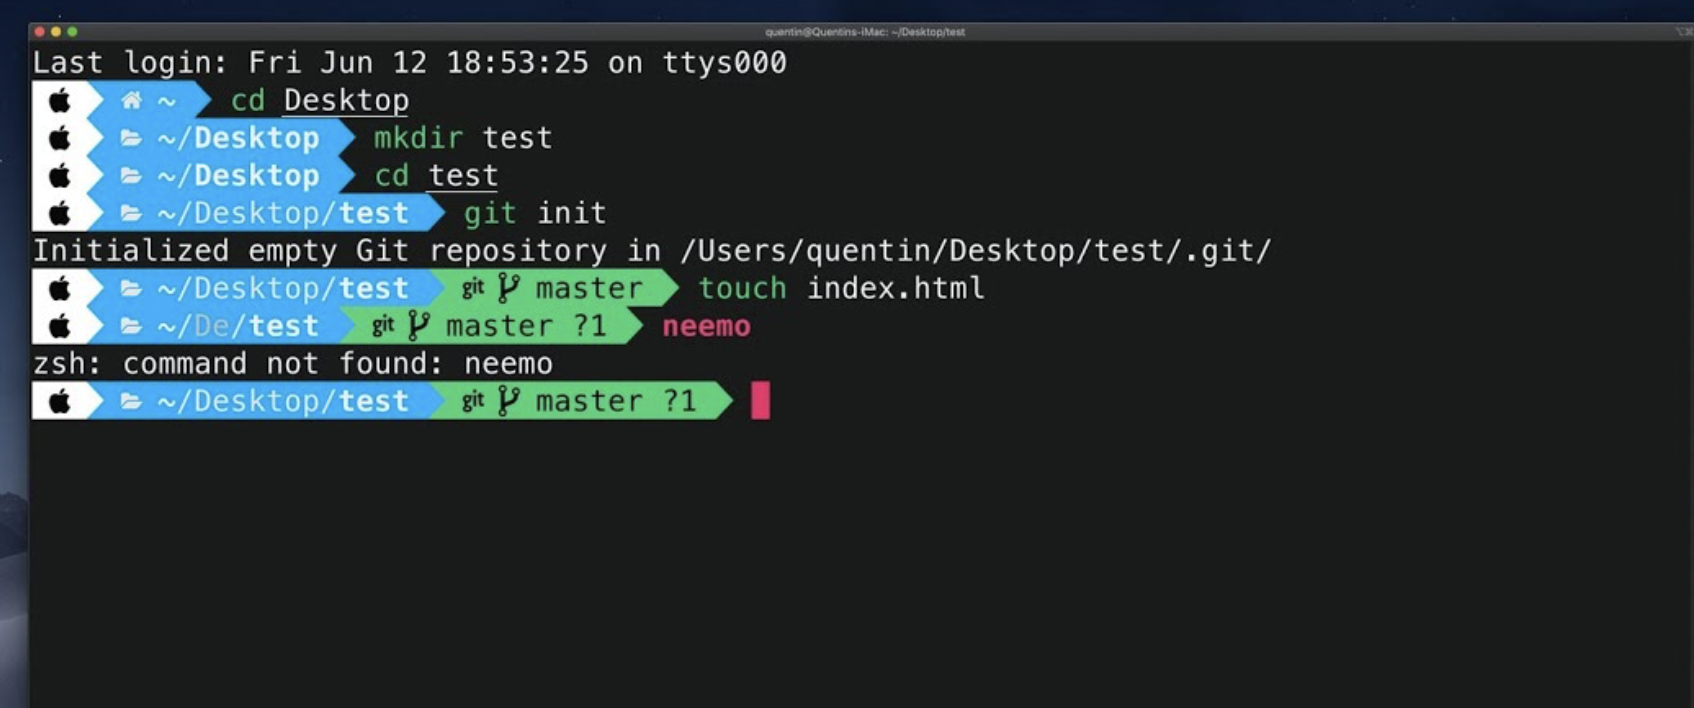
\includegraphics[width=0.9\textwidth]{iterm2.png}
\caption{iTerm2 with Powerlevel10k theme showing git status, conda environment, and more}
\end{figure}

\subsection{Visualization and Diagramming Tools}

\textbf{Advanced Tools for Research Visualization}

\subsubsection{Excalidraw}
\textbf{Website:} \url{https://excalidraw.com/}

Excalidraw is a virtual whiteboard tool that enables you to create beautiful hand-drawn style diagrams effortlessly:
\begin{itemize}
    \item \textbf{Perfect for:} Quick architectural diagrams, flowcharts, and conceptual illustrations
    \item \textbf{Key Features:}
    \begin{itemize}
        \item Hand-drawn aesthetic that's perfect for informal presentations
        \item Real-time collaboration for team brainstorming
        \item Export to PNG, SVG, and clipboard
        \item Works entirely in the browser — no installation needed
    \end{itemize}
    \item \textbf{Research Applications:}
    \begin{itemize}
        \item System architecture sketches during design phase
        \item Algorithm flowcharts for presentations
        \item Brainstorming session visualizations
        \item Quick diagrams for group meetings
    \end{itemize}
\end{itemize}

\subsubsection{PlotNeuralNet}
\textbf{Repository:} \url{https://github.com/HarisIqbal88/PlotNeuralNet}

PlotNeuralNet is a LaTeX-based tool specifically designed for creating publication-quality neural network architecture diagrams:
\begin{itemize}
    \item \textbf{Perfect for:} Research papers, thesis figures, and technical presentations
    \item \textbf{Key Features:}
    \begin{itemize}
        \item Creates professional 3D neural network visualizations
        \item Fully customizable layers and connections
        \item Consistent styling across all diagrams
        \item Generates LaTeX/TikZ code for easy integration
    \end{itemize}
    \item \textbf{Research Applications:}
    \begin{itemize}
        \item CNN/RNN/Transformer architecture illustrations
        \item Paper and thesis figures that meet publication standards
        \item Technical documentation of model architectures
        \item Poster presentations at conferences
    \end{itemize}
    \item \textbf{Pro Tip:} Start with the provided examples and modify them to match your specific architecture — it's much easier than building from scratch!
\end{itemize}

\subsection{System Resource Monitoring and Performance Optimization}

\textbf{Essential Skills for Efficient Development}

As researchers working with data processing and deep learning, monitoring system resources and utilizing parallel processing are critical skills that can dramatically improve your productivity and code efficiency.

\subsubsection{System Resource Monitoring}

\textbf{Why Monitor Resources?}
\begin{itemize}
    \item Identify bottlenecks in data processing pipelines
    \item Detect memory leaks and inefficient code early
    \item Optimize GPU utilization for deep learning tasks
    \item Prevent system crashes from resource exhaustion
    \item Validate that parallel processing is working effectively
\end{itemize}

\textbf{Essential Monitoring Tools:}
\begin{itemize}
    \item \textbf{htop}: Interactive process viewer showing real-time CPU usage per core
    \item \textbf{nvtop}: GPU monitoring for NVIDIA cards (GPU utilization, memory, temperature)
    \item \textbf{gpustat}: Simple command-line GPU status viewer
    \item \textbf{btop}: Modern resource monitor with beautiful graphs and real-time updates
    \item \textbf{nvidia-smi}: Built-in NVIDIA GPU monitoring tool
\end{itemize}

\subsubsection{Parallel Processing for Efficiency}

\textbf{Serial vs Parallel Processing Comparison:}

\begin{verbatim}
Serial Processing:      [Task 1] -> [Task 2] -> [Task 3] -> [Task 4]
                       Time: ================================
                       
Parallel Processing:    [Task 1] [Task 2]
                       [Task 3] [Task 4]
                       Time: ================
                       
Result: ~4x speed improvement (ideal case)
\end{verbatim}

\textbf{Performance Comparison Example:}
\begin{table}[H]
\centering
\begin{tabular}{@{}llll@{}}
\toprule
\textbf{Task} & \textbf{Serial Time} & \textbf{Parallel Time (4 cores)} & \textbf{Speed-up} \\
\midrule
Data preprocessing & 100s & 28s & 3.6x \\
Model training (CPU) & 240s & 65s & 3.7x \\
Batch inference & 60s & 18s & 3.3x \\
Image processing & 180s & 48s & 3.8x \\
\bottomrule
\end{tabular}
\caption{Typical performance gains from parallelization}
\end{table}

\textbf{Practical Implementation Examples:}
\begin{itemize}
    \item \textbf{Python}: Use \texttt{multiprocessing}, \texttt{concurrent.futures}, or \texttt{joblib}
    \item \textbf{NumPy/Pandas}: Vectorized operations instead of loops
    \item \textbf{Deep Learning}: Batch processing, DataLoader with \texttt{num\_workers $>$ 0}
    \item \textbf{Data Processing}: Transform \texttt{map()} → \texttt{parallel\_map()}
\end{itemize}

\subsubsection{Best Practices and Monitoring Guidelines}

\textbf{What to Monitor During Development:}
\begin{itemize}
    \item \textbf{CPU Usage}: Aim for $>$80\% utilization across all cores when parallel processing
    \item \textbf{Memory Usage}: Watch for memory leaks; avoid swapping to disk
    \item \textbf{GPU Utilization}: Should be $>$90\% during deep learning training
    \item \textbf{I/O Wait}: High I/O wait indicates data loading bottlenecks
\end{itemize}

\textbf{Common Parallel Processing Pitfalls:}
\begin{itemize}
    \warningitem I/O bottlenecks limiting parallel gains
    \warningitem Python's GIL (use multiprocessing instead of threading for CPU tasks)
    \warningitem Overhead from creating too many small parallel tasks
    \warningitem Insufficient memory causing thrashing
\end{itemize}

\textbf{Quick Reference Commands:}

\begin{lstlisting}[style=bashstyle, caption=System Monitoring Commands]
# Monitor CPU usage
htop                    # Interactive CPU monitor
top -u                  # Alternative CPU monitor

# Monitor GPU (NVIDIA)
nvidia-smi -l 1        # Updates every 1 second
nvtop                  # Interactive GPU monitor
gpustat -i 1           # Simple GPU status
\end{lstlisting}

\begin{lstlisting}[style=pythonstyle, caption=Python Parallel Processing Example]
# Python parallel example
from multiprocessing import Pool

def process_func(item):
    # Your processing logic here
    return item * 2

with Pool() as p:
    results = p.map(process_func, data_list)
\end{lstlisting}

\textbf{Pro Tips:}
\begin{itemize}
    \item Always benchmark before and after implementing parallelization
    \item Monitor resources during the ENTIRE training process, not just at the start
    \item For deep learning: use \texttt{DataLoader(num\_workers=4-8)} for faster data loading
    \item Check if your bottleneck is CPU, GPU, or I/O before optimizing
\end{itemize}

\vspace{1cm}
\begin{tcolorbox}[colback=gray!10,colframe=gray!50,title=AI Disclosure]
Some text and links in this document were compiled with AI assistance. Please forgive any broken links.
\end{tcolorbox}

\end{document}